\section {Aufbau und Durchführung}
\label{sec:durchführung}

\subsection{Die Hochvakuum-Diode}

\begin{figure}
  \centering
  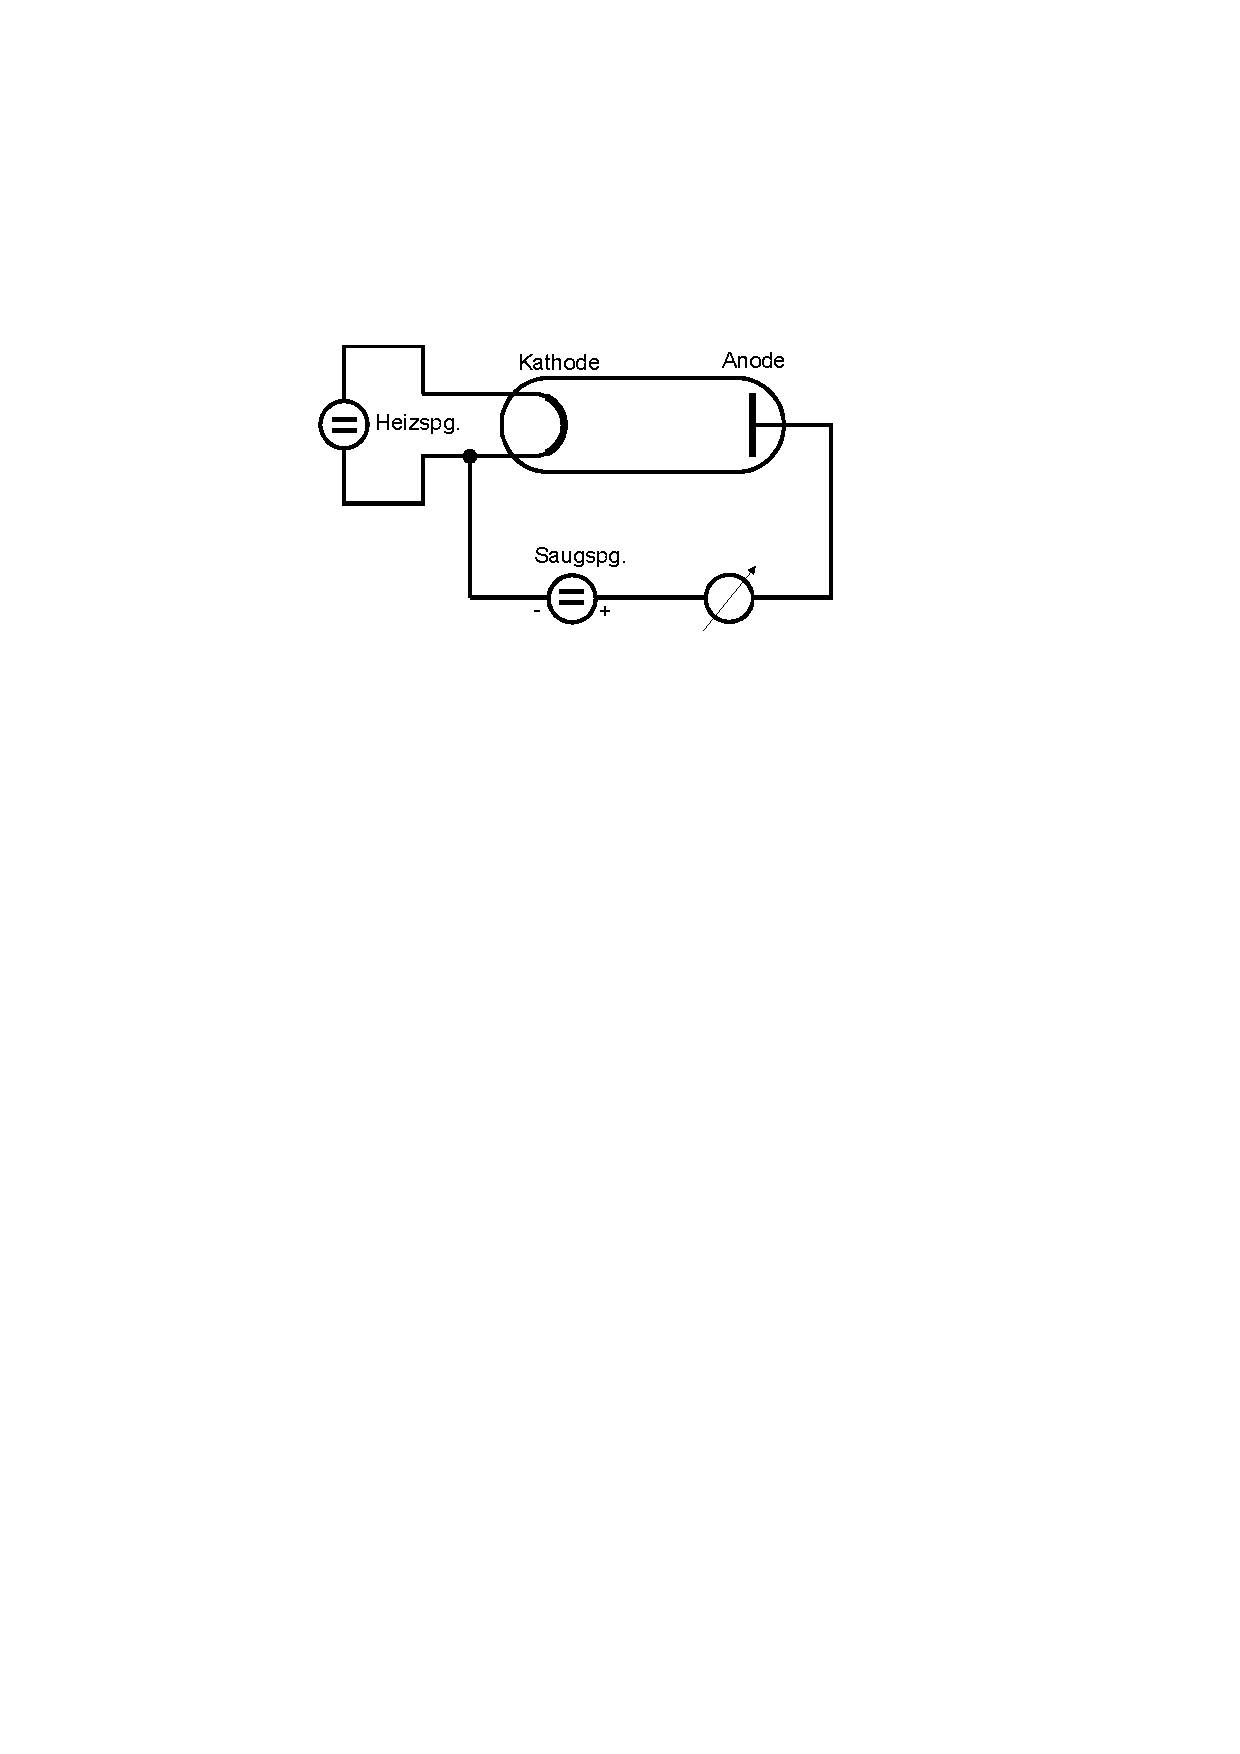
\includegraphics[scale=0.6]{content/diode.pdf}
\caption{Grundsätzliche Beschaltung einer Hochvakuum-Diode \cite{anleitung504}.}
  \label{fig:diode}
\end{figure}

Abbildung \ref{fig:diode} zeigt eine Hochvakuum-Diode, die für alle Messungen verwendet wird, um zu verhindern, dass die freien Elektronen mit den Molekülen der Luft wechselwirken.
In dem evakuierten Glaskörper, befindet sich ein Draht, die Glühkathode, der mittels Strom erhitzt wird, sodass Elektronen emittiert werden. Durch eine zweite Elektrode, die Anode, entsteht ein elektrisches Feld.

\subsection{Aufnahme der Kennlinien der Hochvakuum-Diode}

Um die Diodenkennlinien aufzunehmen, wird die Schaltung aus Abbildung \ref{fig:aufbau1} ohne XY-Schreiber verwendet. Der Heizstrom wird zunächst auf   $I_\mathrm{H} = \SI{2.5}{\ampere}$ eingestellt. Der Wert für die entsprechende Heizspannung, sowie der Wert des Stroms an der Anode werden aufgenommen. Anschließend wird die von außen anliegende Spannung $U$ in \SI{5}{\volt} Schritten von 0 bis 60 \si{\volt}, danach in \SI{10}{\volt} Schritten bis \SI{250}{\volt} erhöht und der dazugehörige Strom an der Anode notiert. Dies wird für die Heizströme $I_\mathrm{H} = \SI{2.4}{\ampere}$, $I_\mathrm{H} = \SI{2.3}{\ampere}$, $I_\mathrm{H} = \SI{2.2}{\ampere}$ und $I_\mathrm{H} = \SI{2.1}{\ampere}$ wiederholt.

\begin{figure}
  \centering
  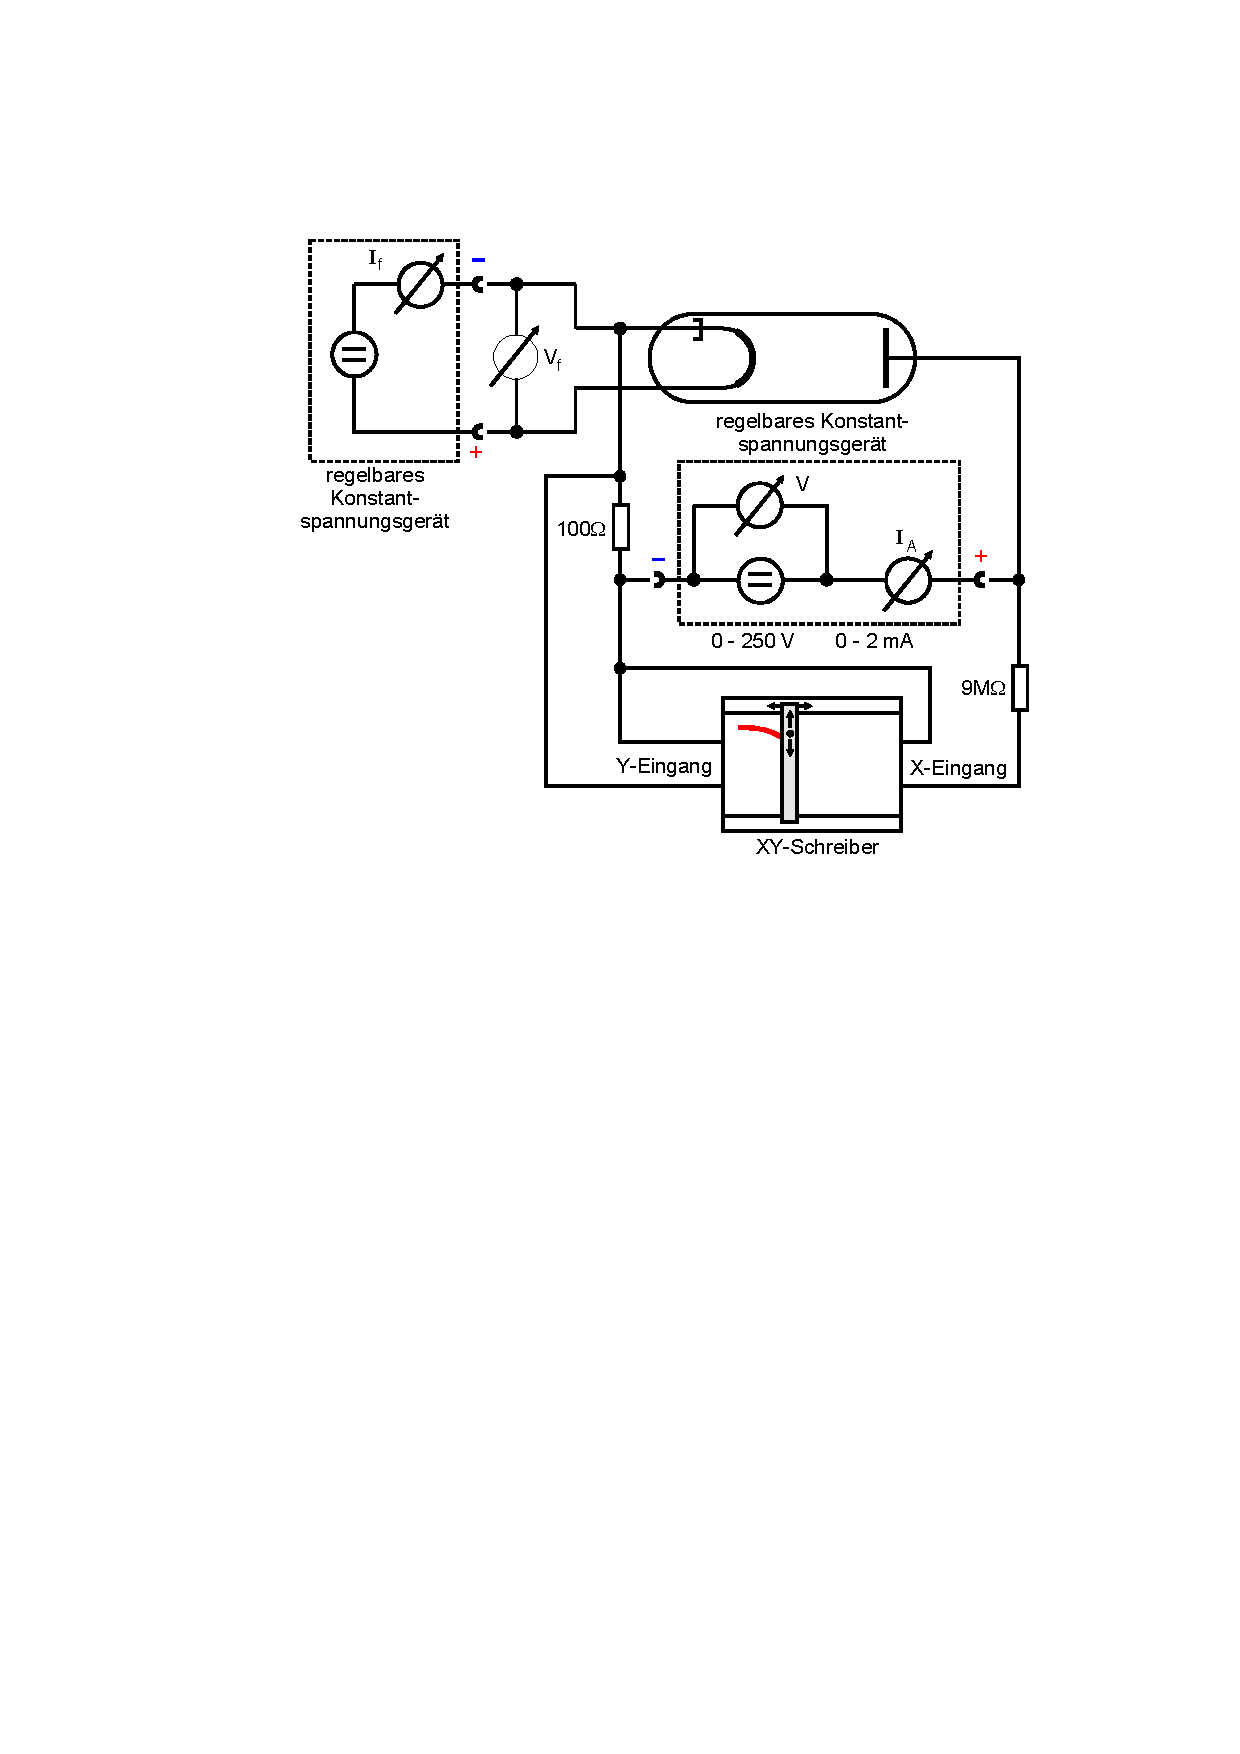
\includegraphics[scale=0.6]{content/aufbau1.pdf}
\caption{Schaltung zur Aufnahme der Diodenkennlinien \cite{anleitung504}.}
  \label{fig:aufbau1}
\end{figure}

\subsection{Aufnahme der Anlaufstromkurve}
\label{sec:anlauf}
\begin{figure}
  \centering
  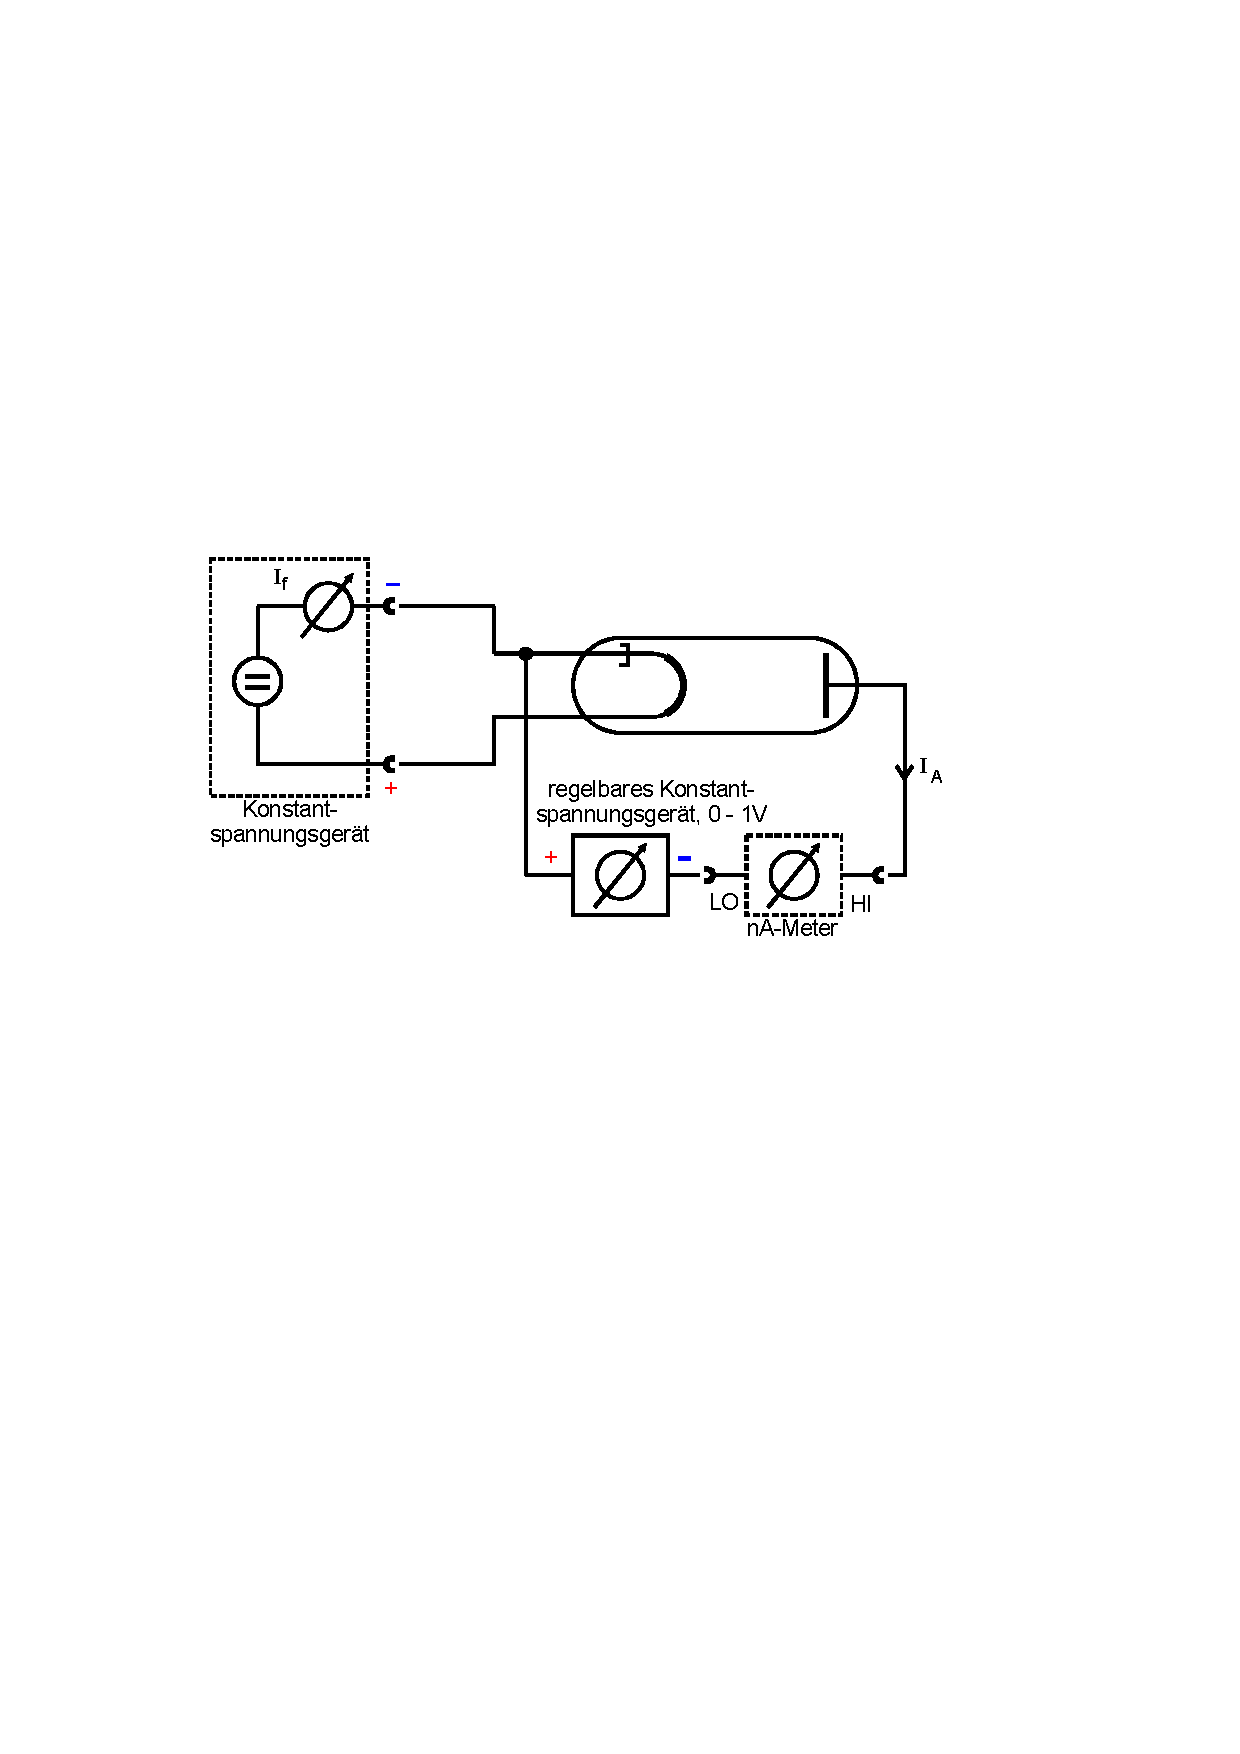
\includegraphics[scale=0.6]{content/aufbau2.pdf}
\caption{Schaltung zur Aufnahme der Anlaufstromkurve \cite{anleitung504}.}
  \label{fig:aufbau2}
\end{figure}

Zur Aufnahme des Anlaufstroms wird die in Abbildung \ref{fig:aufbau2} dargestellte Schaltung aufgebaut. Der Heizstrom beträgt $I_\mathrm{H} = 2,5 \si{\ampere}$. Die Heizspannung wird notiert. Die Gegenspannung $U_G$ wird im Bereich von 0 bis 0,95 \si{\volt} stetig um 0,05 \si{\volt} erhöht und der Strom an der Anode $I_\mathrm{A}$ notiert.
